\chapter{Simulation and Results}
\label{chap4}
In the previous chapter, we have discussed about our methodology for this project while giving details about block diagram, components selection of this project. In this chapter, we will provide source code, and simulation and results of the project.
\section{Simulation Results}
As discussed in the previous chapter in the section of software selection, we have used Proteus to simulate our project.
\section{Circuit Diagram}
Figure \ref{simulation1} shows circuit diagram of the project, which illustrates the main components involved
in Electronic Voting Machine(EVM) Using 8051 Micro-controller. Switches are used to make choices, resister, capacitor, and oscillator are being used to work the micro-controller properly on the circuits with the help of connecting wires.
\begin{figure}[H]  %h=positioning
\begin{center}
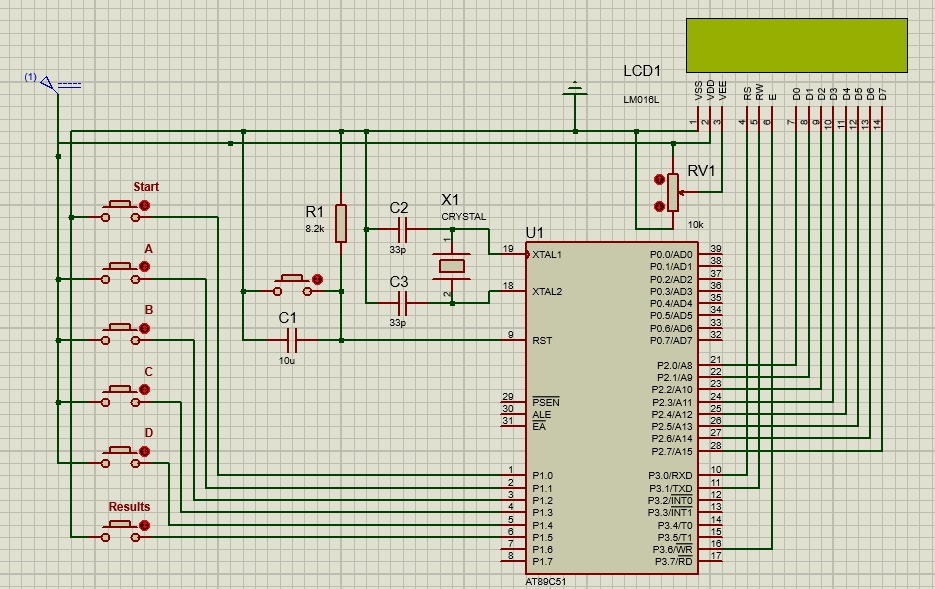
\includegraphics[scale=0.40]{Chapter4/simulation1}
\caption{Circuit Diagram of Electronic Voting Machine(EVM) Using 8051 Microcontroller}
\label{simulation1}
\end{center}
\end{figure}
\section{Source Code}
\begin{lstlisting}[frame=single]
#include<reg51.h>
#define msec 50
#define lcd_data_str_pin P2
sbit rs = P3^0;                  //Register select (RS) pin rs=0 command mode, rs=1 datamode
sbit rw = P3^1;                  //Read write(RW) pin rw=0 write mode, rw=1 read mode
sbit en = P3^6;                  //Enable(EN) pin



sbit ini_pin = P1^0;               // Start voting pin
sbit stop_pin = P1^5;            // Stop voting pin
sbit candidate_1=P1^1;                //Candidate1
sbit candidate_2=P1^2;              //Candidate2
sbit candidate_3=P1^3;                //Candidate3
sbit candidate_4=P1^4;             //Candidate4



int max = 0;
int carry = 0;
int arr[4];             //arry ofsize 4

int vote_amt[3],j;
unsigned int vote_1,vote_2,vote_3,vote_4;

void delay(int delay_time)                           // Time delay function
{

int j,k;
for(j=0;j<=delay_time;j++)
for(k=0;k<=1275;k++);
}

void lcd_cmd(unsigned char cmd_addr)                       //Function to send command to LCD
{
lcd_data_str_pin = cmd_addr;
en = 1;
rs = 0;
rw = 0;
delay(1);
en = 0;
return;
}

void lcd_data_str(char str[50])                               //Function to send string
{
int p;
for (p=0;str[p]!='\0';p++)
{
lcd_data_str_pin = str[p];
rw = 0;
rs = 1;
en = 1;

delay(1);
en = 0;
}
return;
}

void lcd_data_int(unsigned int vote)                        //Function to send 0-9 character values
{
char dig_ctrl_var;
int p;
for (j=2;j>=0;j--)
{
vote_amt[j]=vote%10;
vote=vote/10;
}

for (p=0;p<=2;p++)
{
dig_ctrl_var = vote_amt[p]+48;
lcd_data_str_pin = dig_ctrl_var;
rw = 0;
rs = 1;
en = 1;
delay(1);
en = 0;

}
return;
}

void vote_count()                                               // Function to count votes
{
while (candidate_1==0 && candidate_2==0 && candidate_3==0 && candidate_4==0);
if (candidate_1==1)
{
while (candidate_1 == 1);
{
vote_1 = vote_1 + 1;
}
}

if (candidate_2==1)
{
while (candidate_2 == 1);
{
vote_2 = vote_2 + 1;
}
}

if (candidate_3==1)
{
while (candidate_3 == 1);
{
vote_3 = vote_3 + 1;
}
}

if (candidate_4==1)
{
while (candidate_4 == 1);
{
vote_4 = vote_4 + 1;
}
}
}

void lcd_ini()
{
lcd_cmd(0x38);        //5x7 matrix 2 lines
delay(msec);
lcd_cmd(0x0E);                  //cursor on
delay(msec);
lcd_cmd(0x01);               //clear screen
delay(msec);
lcd_cmd(0x81);                //cursor position to 1st
delay(msec);
lcd_data_str("welcome here");
delay(100);
lcd_cmd(0x01);           //clear
delay(msec);
lcd_cmd(0x80);             //cursor position to 0 of line 1
delay(msec);
lcd_data_str( "you" );
delay(msec);
lcd_cmd(0x14);                     //space between
delay(msec);
lcd_data_str("can now");
delay(msec);
delay(msec);
lcd_cmd(0xC0);                 // second line
delay(msec);
lcd_data_str("cast your");
delay(msec);
lcd_cmd(0x14);                 // space
delay(msec);
lcd_data_str("vote");
delay(100);
lcd_cmd(0x01);                 //clear lcd
delay(msec);
lcd_cmd(0x80);                 //cursor position to 0 of line 1
delay(msec);
lcd_data_str("A");
delay(msec);
lcd_cmd(0x84);               // 4th col
delay(msec);
lcd_data_str("B");
delay(msec);
lcd_cmd(0x88);               // 8th col
delay(msec);
lcd_data_str("C");
delay(msec);
lcd_cmd(0x8C);                 // 12 col
delay(msec);
lcd_data_str("D");
delay(msec);
vote_count();
lcd_cmd(0x01);              //clear lcd
delay(msec);
lcd_cmd(0x83);             //ist line 3rd col
delay(msec);
lcd_data_str("thank");
delay(msec);
lcd_cmd(0x14);                 //space
delay(msec);
lcd_data_str("you");
delay(100);
}

void results()                // Function to show results
{
int i;
carry = 0;
lcd_cmd(0x01);                           //clear lcd
delay(msec);
lcd_cmd(0x80);                           //cursor position to 0 of line 1
delay(msec);
lcd_data_str("results");
delay(msec);
lcd_cmd(0x14);                        //space
delay(msec);
lcd_data_str("are");
delay(msec);
lcd_cmd(0x14);                         //space
delay(msec);
lcd_data_str("out");
delay(msec);
lcd_cmd(0x01);                         //clear lcd
delay(msec);
lcd_cmd(0x80);                         //cursor position to 0 of line 1
delay(msec);
lcd_data_str("A");
delay(msec);
lcd_cmd(0x84);                          //4th col
delay(msec);
lcd_data_str("B");
delay(msec);
lcd_cmd(0x88);                          // 8th col
delay(msec);
lcd_data_str("C");
delay(msec);
lcd_cmd(0x8C);                          // 12th col
delay(msec);
lcd_data_str("D");
delay(msec);
lcd_cmd(0xC0);                    //second line
delay(100);

lcd_data_int(vote_1);
delay(msec);
lcd_cmd(0xC4);                      //jump to 2nd line 4th row
delay(msec);
lcd_data_int(vote_2);
delay(msec);
lcd_cmd(0xC8);                      // 2nd line 8th row
delay(msec);
lcd_data_int(vote_3);
delay(msec);
lcd_cmd(0xCC);                   // 2nd line 12th row
delay(msec);
lcd_data_int(vote_4);
delay(300);

arr[0] = vote_1;                      //arry ofsize 4
arr[1] = vote_2;
arr[2] = vote_3;
arr[3] = vote_4;

for( i=0; i<4; i++)
{
if(arr[i]>=max)
max = arr[i];
}

if ( (vote_1 == max) && ( vote_2 != max) && (vote_3 != max)&& (vote_4 != max) )
{

carry = 1;
lcd_cmd(0x01);            //clear lcd
delay(msec);
lcd_cmd(0x80);              //cursor position to 0 of line 1
delay(msec);
lcd_data_str("congratulations");
delay(50);
lcd_cmd(0xC4);        //jump to 2nd line 4th col
delay(msec);
lcd_data_str("A");
delay(msec);
lcd_cmd(0x14);               //space
delay(msec);
lcd_data_str("wins");
delay(msec);
}

if ( (vote_2 == max) && ( vote_1 != max) && (vote_3 != max)&& (vote_4 != max) )
{
carry = 1;
lcd_cmd(0x01);     //clear lcd
delay(msec);
lcd_cmd(0x80);           //cursor position to 0 of line 1
delay(msec);
lcd_data_str("congratulations");
delay(50);
lcd_cmd(0xC4);                               //jump to 2nd line 4th col
delay(msec);
lcd_data_str("B");
delay(msec);
lcd_cmd(0x14);                 //space
delay(msec);
lcd_data_str("wins");
delay(msec);
}

if ( (vote_3 == max) && ( vote_2 != max) && (vote_1 != max)&& (vote_4 != max) )
{
carry = 1;
lcd_cmd(0x01);               //clear lcd
delay(msec);
lcd_cmd(0x80);                         //cursor position to 0 of line 1
delay(msec);
lcd_data_str("congratulations");
delay(50);
lcd_cmd(0xC4);                           ////jump to 2nd line 4th col
delay(msec);
lcd_data_str("C");
delay(msec);
lcd_cmd(0x14);                  //space
delay(msec);
lcd_data_str("wins");
delay(msec);
}

if ( (vote_4 == max) && ( vote_2 != max) && (vote_3 != max)&& (vote_1 != max) )
{
carry = 1;
lcd_cmd(0x01);     //clear lcd
delay(msec);
lcd_cmd(0x80);                          //cursor position to 0 of line 1
delay(msec);
lcd_data_str("congratulations");
delay(50);
lcd_cmd(0xC4);                      //jump to 2nd line 4th col
delay(msec);
lcd_data_str("D");
delay(msec);
lcd_cmd(0x14);                  //space
delay(msec);
lcd_data_str("wins");
delay(msec);
}

if (carry==0)

{
lcd_cmd(0x01);                 //clear lcd
delay(msec);
lcd_cmd(0x82);                //ist line 2nd col
delay(msec);
lcd_data_str("clash");
delay(50);
lcd_cmd(0x14);               //space
delay(msec);
lcd_data_str("between");
delay(50);
if(vote_1 == max)
{
lcd_cmd(0xC2);              //2nd line 2nd col
lcd_data_str("A");
delay(50);
}
if(vote_2 == max)
{
lcd_cmd(0xC5);                  //2nd line 5th col
lcd_data_str("B");
delay(50);
}
if(vote_3 == max)
{
lcd_cmd(0xC9);                      //2nd line 9th col
lcd_data_str("C");
delay(50);
}
if(vote_4 == max)
{
lcd_cmd(0xCD);                          //2nd line 12th col
lcd_data_str("D");
delay(50);
}
}
}

void main()
{
ini_pin = stop_pin = 1;
vote_1 = vote_2 = vote_3 = vote_4 = 0;
candidate_1 = candidate_2 = candidate_3 = candidate_4 = 0;
lcd_cmd(0x38);               //5x7 matrix 2 lines
delay(msec);
lcd_cmd(0x0E);               //cursor on
delay(msec);
lcd_cmd(0x01);                 //clear lcd
delay(msec);
lcd_cmd(0x80);              //cursor to fisrt pos
delay(msec);
lcd_data_str( "press b1" );
delay(msec);
lcd_cmd(0x14);               //sapce
delay(msec);
lcd_data_str("to");
delay(msec);
lcd_cmd(0xC0);                 // second line
delay(msec);
lcd_data_str("start");
delay(100);
while(1)
{
while(ini_pin != 0)
{
if (stop_pin == 0)
break;
}
if (stop_pin == 0)            //result pin
{
break;
}
lcd_ini();
}

while(1)
{
results();
}
}
\end{lstlisting}
\clearpage
\section{Results}
Following screen shot will show the step wise results which showed up as we run the project.
\begin{figure}[H]  %h=positioning
\begin{center}
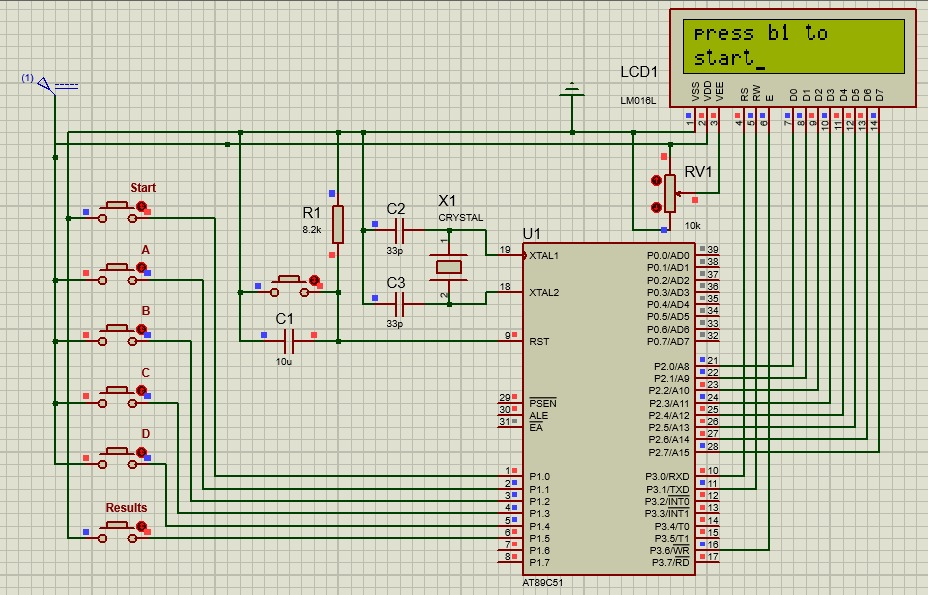
\includegraphics[scale=0.50]{Chapter4/simulation3}
%\caption{Circuit Diagram of Electronic Voting Machine(EVM) Using 8051 Microcontroller}
%\label{simulation1}
\end{center}
\end{figure}
\begin{figure}[H]  %h=positioning
\begin{center}
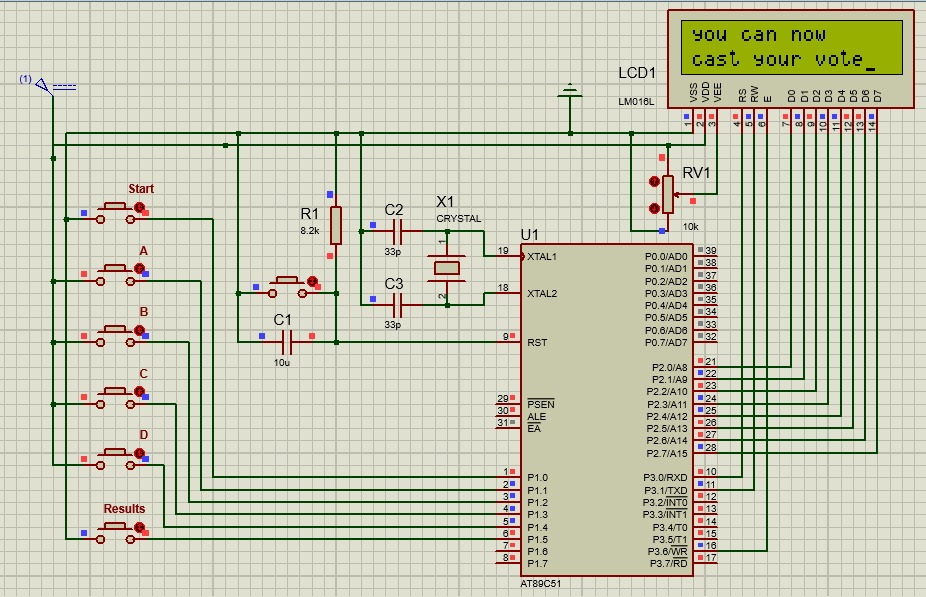
\includegraphics[scale=0.50]{Chapter4/simulation4}
%\caption{Circuit Diagram of Electronic Voting Machine(EVM) Using 8051 Microcontroller}
%\label{simulation1}
\end{center}
\end{figure}
\begin{figure}[H]  %h=positioning
\begin{center}
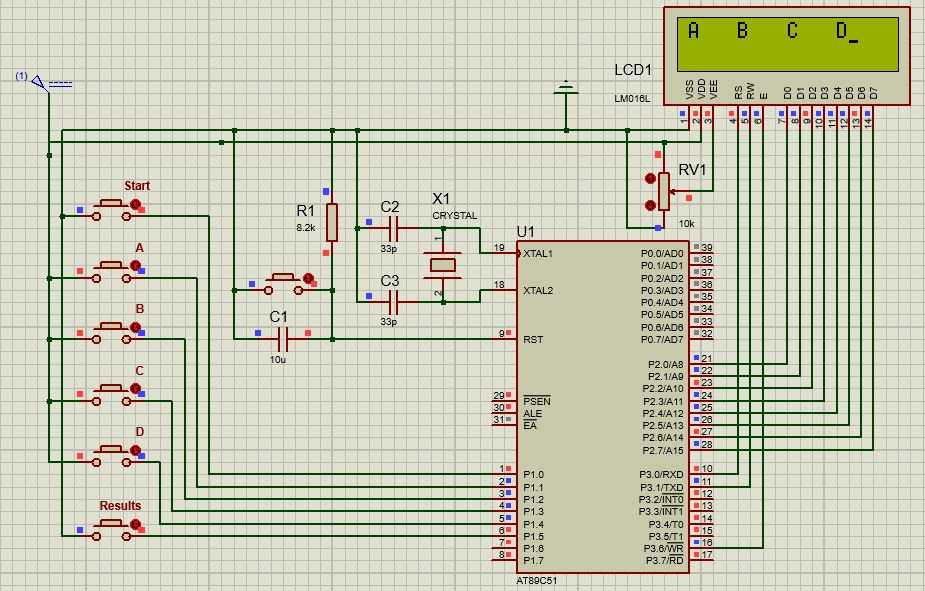
\includegraphics[scale=0.50]{Chapter4/simulation5}
%\caption{Circuit Diagram of Electronic Voting Machine(EVM) Using 8051 Microcontroller}
%\label{simulation1}
\end{center}
\end{figure}
\begin{figure}[H]  %h=positioning
\begin{center}
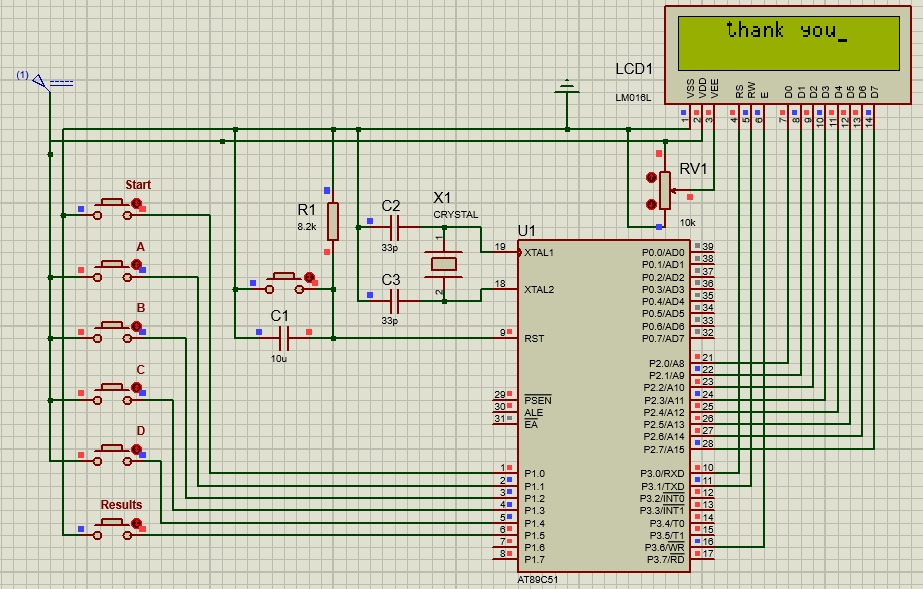
\includegraphics[scale=0.50]{Chapter4/simulation6}
%\caption{Circuit Diagram of Electronic Voting Machine(EVM) Using 8051 Microcontroller}
%\label{simulation1}
\end{center}
\end{figure}
\begin{figure}[H]  %h=positioning
\begin{center}
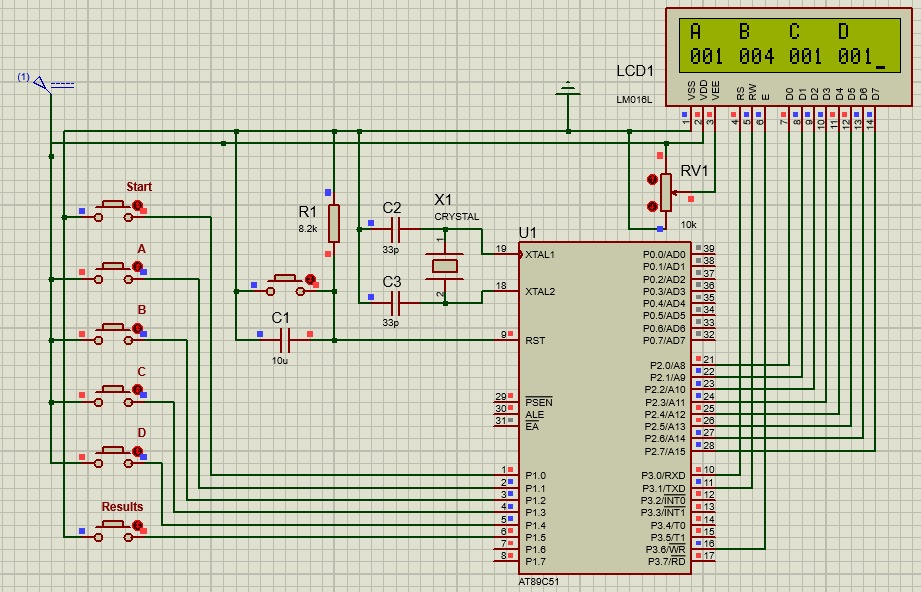
\includegraphics[scale=0.50]{Chapter4/simulation7}
%\caption{Circuit Diagram of Electronic Voting Machine(EVM) Using 8051 Microcontroller}
%\label{simulation1}
\end{center}
\end{figure}
\begin{figure}[H]  %h=positioning
\begin{center}
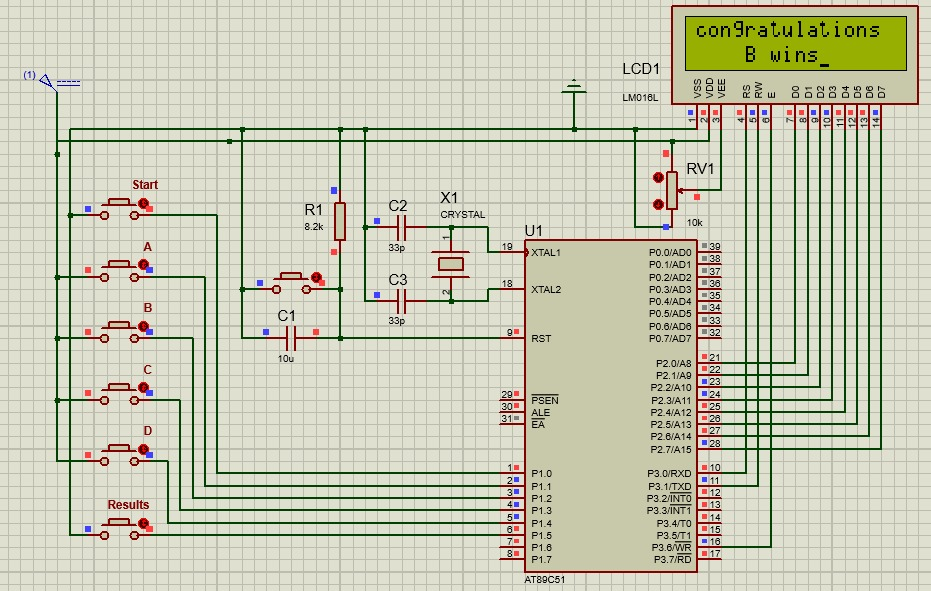
\includegraphics[scale=0.50]{Chapter4/simulation8}
%\caption{Circuit Diagram of Electronic Voting Machine(EVM) Using 8051 Microcontroller}
%\label{simulation1}
\end{center}
\end{figure}
\begin{figure}[H]  %h=positioning
\begin{center}
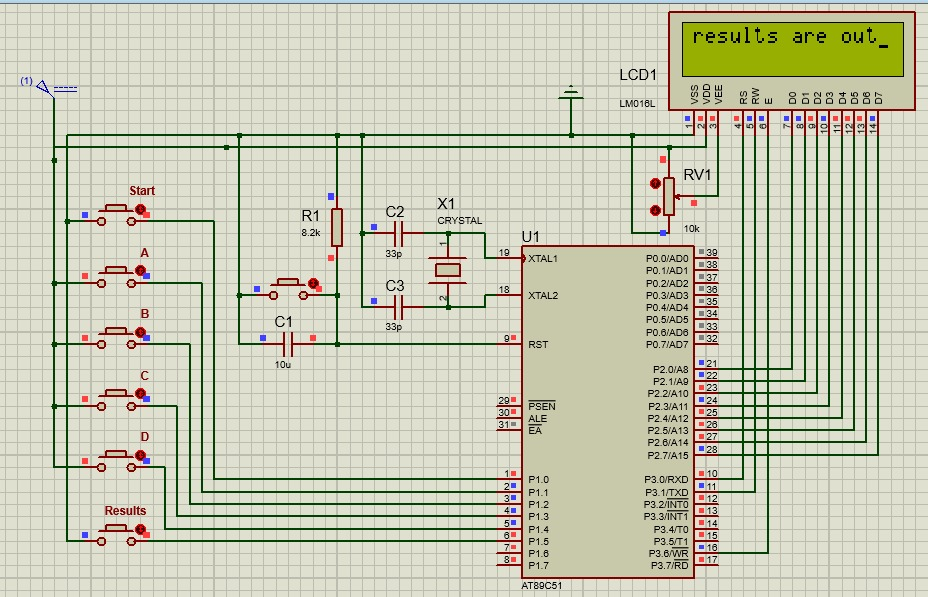
\includegraphics[scale=0.50]{Chapter4/simulation9}
%\caption{Circuit Diagram of Electronic Voting Machine(EVM) Using 8051 Microcontroller}
%\label{simulation1}
\end{center}
\end{figure}

